\documentclass[pra,
superscriptaddress,
 amsmath,amssymb,
 aps,twocolumn]{revtex4-1}


\usepackage{graphicx}% Include figure files
\usepackage{dcolumn}% Align table columns on decimal point
\usepackage{bm}
% \usepackage[all]{nowidow}
\usepackage{hyperref}
\hypersetup{colorlinks = true, linkcolor = [rgb]{0.19411,0.51882,0.667058}, urlcolor = [rgb]{0.125490,0.29542,0.1647058}, citecolor = [rgb]{0.75882,0.37411,0.14117}}


\widowpenalty10000
% \clubpenalty10000


\graphicspath{{../images/}}

\usepackage[toc,page]{appendix}

\newcommand{\nn}{\nonumber \\}
\newcommand{\bra}[1]{\langle{#1}|}
\newcommand{\ket}[1]{|{#1}\rangle}
\newcommand{\braket}[2]{\langle{#1}|{#2}\rangle}
%\def\comment#1{}
\def\comment#1{ [{\bf Comment:} {\sf #1}]}
\def\labell#1{\label{#1}}
%\def\labell#1{\label{#1}{\mbox{{\tiny #1}}}}
% \def\sectionp#1{{\par\em #1:--- }}
% \def\mostra#1{\refstepcounter{#1}\arabic{#1}}
\def\togli#1{}
\def\tr{\mbox{Tr}}
\def\iden{\openone}
\def\>{\rangle}
\def\<{\langle}


\usepackage{braket}

\def\>{\rangle}
\def\<{\langle}

% \def\section#1{{\par\em #1:--- }}
\usepackage[bottom]{footmisc}


\begin{document}
% \fbox{{\scriptsize Internal report \today}}

\title{Continuous variable }




\begin{abstract}

\end{abstract}

\date{\today}

\maketitle

% 
\section{Motivation}


Up to this moment we have considered systems with a discrete number of dimensions, we now consider a 
system with continuous variables, i.e. an infinite number of dimensions, which is based on the quantum harmonic oscillator. The main motivation for using continuous variables, however, comes from the fact that all the main quantum information protocols can be implemented efficiently in an experiment \cite{bib:RevModPhys.77.513}.


Here we focus on optical Gaussian states as they are the natural choice for communication protocols. Before delving into quantum communication and computation, in Sec.~\ref{basics} we first intoduce the basic tools of quantum optics.


\section{Continuous variables in quantum optics \label{basics}}



In quantum optics, the quantized electromagnetic modes correspond to to quantum harmonic oscillators. Unlike for classical harmonic oscillators, in quantum mechanics, the position and momentum observables are non-commuting Hermitian operators:


\begin{eqnarray}
[\hat x, \hat p] = i \hbar
\end{eqnarray}

For each single mode $k$, the Hamiltonian for a quantum harmonic oscillator is

\begin{align}
\hat H_k  &= \frac{1}{2}(\hat p^2_k + \omega_k \hat x^2_k) \\
		  &= \hbar \omega_k(\hat a^\dagger _k \hat a_k + \frac{1}{2}) \\
		  & = \hbar \omega_k ( n + \frac{1}{2})
\end{align}

\noindent where $n$ corresponds to the number of quanta of energy of the oscillator. The creation and annihilation operators can be written in terms of the $\hat x_k$ and $p_k$ operators

\begin{align}
\hat a^\dagger_k &= \frac{1}{\sqrt{2\hbar \omega_k}}(\omega_k \hat x_k - i \hat p_k), \\ 
\hat a_k         &= \frac{1}{\sqrt{2\hbar \omega_k}}(\omega_k \hat x_k + i \hat p_k),
\end{align}

\noindent or conversely

\begin{align}
\hat x_k &=    \sqrt{\frac{\hbar}{2 \omega_k}}(\hat a_k + \hat a_k^\dagger),   \\
\hat p_k &= -i \sqrt{\frac{\hbar  \omega_k}{2}}(\hat a_k - \hat a_k^\dagger). 
\end{align}

\noindent The position and momentum operators represent the quadratures of a the mode, and correspond to the 
real and imaginary parts of the oscillator's amplitude, see Fig.~\ref{fig:x_and_p}.


\begin{figure}[h!]
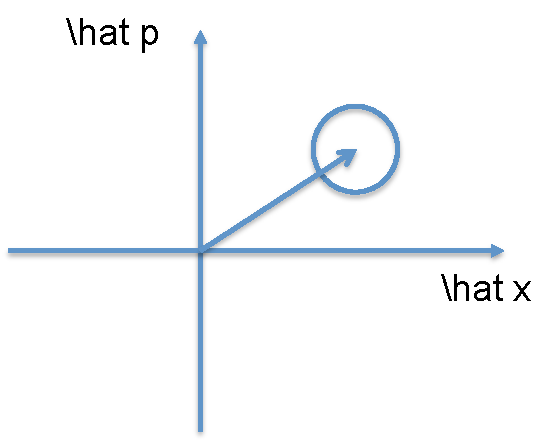
\includegraphics[trim = 0cm 0cm 0cm 0cm, clip, width=0.7\linewidth]{x_and_p.pdf}
\caption{\label{fig:x_and_p} Representation of a state vector in phase space with position ($\hat x$) and momentum ($\hat p$) quadratures. The circle indicates the uncertainty associated with the quadrature, where the Heisenberg uncertainty principle imposes that $\Delta x \Delta p \geq \hbar/2$. }
\end{figure}


The position representation corresponds to expressing a state vector $\ket{\psi}$ in the position basis:
% 
\begin{align}
\ket{\psi} =\int dx \braket{x|\psi} \ket{x} = \int dx \psi(x)\ket{x},
\end{align}
\noindent where $\ket{x}$ is the eigenstate of the position operator. Here the wave function in the position representation is defined as
% 
\begin{align}
\psi(x) = \braket{x|\psi}.
\end{align}
% 

\noindent Let us now find the wavefunction.
Since $\hat a \ket{0} = 0$, we know that

\begin{align}
\frac{1}{\sqrt{2}}(\sqrt{m \omega} 
\hat x + \frac{1}{\sqrt{m \omega}} i 
\hat p)\ket{0} = 0.
\end{align}

\noindent Given $\psi_0(x) = \braket{x|0}$,
\begin{align}
			& (m \omega x + \frac{d}{dx}) \psi_0(x) =0 \\
\rightarrow  \; &\psi_0(x) \propto e^{- m \omega x^2/2}.
\end{align}

\noindent The other position eigenstates can be built using Hermite Polynomials $H_n(x)$, with solutions

\begin{align}
\psi_n (x) = \braket{x|n} = \frac{1}{\sqrt{2^n n!}} H_n(x) \psi_0 (x).
\end{align}

The quadrature eigenstates are mutually related to each other by a Fourier transform:

\begin{align}
\ket{x} = \frac{1}{\sqrt{\pi}} \int_{-\infty} ^\infty e^{-2 i x p} \ket{p} dp,\\
\ket{p} = \frac{1}{\sqrt{\pi}} \int_{-\infty} ^\infty e^{+2 i x p} \ket{x} dx.\\
\end{align}

\noindent It is worth mentioning that the quadrature eigenstates are unphysical and unormalized, but they are very useful in performing the idealized quantumn information protocols.


\section{Unitary operators in CV}



\subsection{The displacement operator}
The one-mode displacement operator generates the coherent states from vacuum.
\begin{align}
D(\alpha) = e^{\alpha \hat a^\dagger - \alpha^* 
\hat a}.
\end{align}
An important property (BCH)
\begin{align}
D(\alpha) = e^{-|\alpha|^2/2} e^{\alpha 
\hat a^\dagger} e^{-\alpha^* 
\hat a}
\end{align}
This acts on the vacuum to give the coherent state, here $\ket{0}$ denotes a vacuum state.

\begin{align} \displaystyle
\ket{\alpha} &= D(\alpha) \ket{0}\\
			 &= e^{-|\alpha|^2/2} e^{\alpha 
\hat a^\dagger}\ket{0} \\
			 &= e^{-|\alpha|^2/2} \sum_{n=0}^\infty \frac{\alpha^n}{\sqrt{n!}}\ket{n}
\end{align}


\subsection{Phase rotation}
Another important feature in the CV formalism is the phase degree of freedom. The phase of an
electromagnetic field has no meaning on its own, and is usually defined with respect to a strong local oscillator.
The phase rotation operator is given by 
\begin{align}
R(\theta) = e^{i\theta(\hat a^\dagger \hat a) }
\end{align}
In the Heisenberg picture,
\begin{align}
R^\dagger(\theta) a R(\theta) = a e^{-i\theta},
\end{align}

\noindent and the more general quadrature operators 
\begin{eqnarray}
\hat x ^{\theta} = \hat a e^{-i \varphi} + \hat a^\dagger e^{-i\varphi}\\
\hat p ^{\theta} = \hat a e^{-i \varphi} - \hat a^\dagger e^{-i\varphi}
\end{eqnarray}
\noindent can be obtained by applying $R(\theta)$. They transform as
\begin{eqnarray}
\begin{pmatrix}
\hat x ^{\theta}\\
\hat p ^{\theta}

\end{pmatrix}
=
\begin{pmatrix}
\hat \cos(\theta) & \sin(\theta) \\
\hat -\sin(\theta) & \cos(\theta)
\end{pmatrix}
\begin{pmatrix}
\hat x\\
\hat p
\end{pmatrix}.
\end{eqnarray}



\subsection{Entanglement generation}


The essential ingredient to generate entanglement in CV is squeezed light. A widely used method for generating single photons is via spontaneous parametric down conversion in a nonlinear medium \cite{bib:PhysRevLett.75.4337, bib:o2009photonic}. Here, a ``classical" (i.e. strong) electromagnetic field drives the medium, and pairs of correlated photons of the same frequency can be generated.
The effective Hamiltonian of one such process can be written as

\begin{equation}
H = \epsilon {\hat a_1}^\dagger  \hat a_{2} ^\dagger + \epsilon^* \hat a_1 \hat a_2,
\end{equation}
\noindent $\epsilon$ is the amplitude of the driving field strength.
% 


\subsubsection{One-mode squeezing}
The one-mode squeeze operator is given by

\begin{align}
\hat S(\zeta) = \text{exp} (\zeta^* \frac{\hat   a ^2}{2} -\zeta \frac{\hat  a ^{\dagger 2} }{2})
\end{align}

\noindent where $\zeta  = r e^{i \phi}= - i \epsilon t/h $, $r$ is known as the squeeze parameter, which will determine the size of the squeezing and $\varphi \in [0, 2\pi]$. The parameter $\zeta$ is a function of the int feraction time (i.e. length of the medium), the amplitude of the driving field strength $\epsilon$.

The creation and annihilation operators transform under the squeezing operator in the following way

\begin{align}
\hat S^\dagger(\zeta) \hat a S(\zeta) &= \hat a \cosh r - \hat a^\dagger e^{i \theta}\sinh r \\
% 
\hat S^\dagger(\zeta) \hat a^\dagger S(\zeta) &= \hat a ^\dagger \cosh r - \hat a  e^{-i \theta} \sinh r
\label{eq:squeezeannihilation}
\end{align}

\noindent These can be derived from the Baker–Campbell–Hausdorff (BCH) relations, here we derive the first equation in \eqref{eq:squeezeannihilation}. Firstly, we need the following BCH identity:
% 
\begin{eqnarray}
e^X Y e^{-X} &=& Y + [X,Y] + \frac{1}{2!}[X,[X,Y]] \nonumber \\
             &+& \frac{1}{3!}[X,[X,[X,Y]]]+ ...
\end{eqnarray}


% 
\begin{align} \displaystyle
\hat S^\dagger(\zeta) =& \hat S^\dagger(\zeta) \hat a  \hat  S(\zeta) \nonumber\\
					  =& \hat  a + \underbrace{[ \zeta \frac{\hat a^{\dagger2}}{2}-\zeta^*\frac{\hat  a^2}{2}, \hat a  ]}
					  _{= -\zeta\hat   a^\dagger}  + \nonumber\\
% 
					  & \frac{1}{2!} \underbrace{[\zeta \frac{\hat  a^{\dagger2} }{2}-\zeta^*\frac{ \hat  a^2}{2}, -\zeta \hat a^\dagger]}_{= \zeta^* \zeta \hat  a} + \nonumber\\
					  & \frac{1}{3!}
					  [\zeta \frac{\hat  a^{\dagger2} }{2}-\zeta^*\frac{\hat  a^2}{2}, +|\zeta|^2 \hat  a] \nonumber\\
					 =& \sum_m \frac{|\zeta|^{2m}}{(2m)!} \hat  a -  \frac{|\zeta|^{2m} \zeta}{(2m+1)!} \hat a^\dagger  \nonumber\\
					 =& \hat a \cosh|\zeta| -\hat  a^\dagger \sinh |\zeta| e^{i \theta}.
\end{align}

If we choose $\theta = 0$, the quadrature operators transform as

\begin{eqnarray}
\hat x  &=& \sqrt{\frac{\hbar}{2 \omega}} (\hat a+\hat a^\dagger) \\
    &\rightarrow& 
   \sqrt{\frac{\hbar}{2 \omega}}\hat    S^\dagger(\zeta) (\hat a+ \hat a^\dagger) \hat S(\zeta)\\
  &=&\sqrt{\frac{\hbar}{2 \omega}}  (\hat a \cosh r - \hat a^\dagger  \sinh r +\\
                                  & &\hat a^\dagger \cosh r - \hat a  \sinh r)\\
   &=&\hat x e^{-r},\\
\hat p &\rightarrow& \hat p e^{r}.
\end{eqnarray}

\noindent That is, the squeezing operator amplifies (the uncertainty of) one quadrature at the expense of the other.


If we want to write $\hat S(\zeta)\ket{0}$ in the photon number basis, we need to express $\hat S(\zeta)$ in a more convenient form. It can be shown \cite{bib:helgason1962differential} that if the operators $\hat A$ and $\hat B$ obey the commutation relations 
\begin{eqnarray}
[\hat A,\hat B] = \hat H, \quad [\hat H,\hat A] = 2 \hat B, \qquad [\hat H, \hat B] = 2 \hat A
\end{eqnarray}
% 
\noindent then
\begin{eqnarray}
e^{t(\hat A+\hat B)} = e^{\tanh r \hat B} e^{\log(\cosh t) \hat H } e^{\tanh t \hat A }
\end{eqnarray}

\noindent If we choose
\begin{eqnarray}
X = \hat a ^2  e^{-i\theta}/2, \qquad
Y = -\hat a ^\dagger e^{i \theta} /2,
\end{eqnarray}

\noindent the squeeze operators can now be factored into a product of exponentials
\begin{eqnarray}
 &&\exp(-  (\hat a ^\dagger)^2  e^{ i \theta} \tanh r /2) \times\\
				  &&\exp[-\frac{1}{4}[\hat a^2 \hat (a^\dagger) ^2 - (\hat a ^\dagger) ^2 
				  \hat  a ^2] \log(\cosh r)] \times \nonumber \\
				  &&\exp(\hat a^2  e^{ i\theta} \tanh r/2 ). \nonumber 
\end{eqnarray}

\noindent Using the commutation relation
% 
\begin{eqnarray}
[a_i,a_j^\dagger] = \delta_{ij},
\end{eqnarray}
after some simple algebra, it can be shown that
\begin{eqnarray}
\hat S(\zeta)\ket{0} = \frac{1}{\sqrt{\cosh r}} \sum_{n=0}^\infty  (\tanh r)^n \frac{\sqrt{(2n)!}}{2^n n!}\ket{2n}.
\end{eqnarray}

\subsubsection{Two-mode squeezing}
The two-mode squeeze operator is then given by
\begin{equation}
\hat S_{12}(\zeta) = \text{exp} (\zeta^* \hat a_1 \hat a_2  - \zeta \hat a_1^\dagger \hat a_2 ^\dagger )
\end{equation}
\noindent
% 
% 
% 
It can be easily verified that the creation/annihilation operators for mode 1 and 2 transform under the operator as

\begin{eqnarray}
S_{12}(\zeta)^\dagger a_1 S_{12}(\zeta) = \hat a_1 \cosh r - \hat a_2^\dagger
e^{i \theta}\sinh r\\
S_{12}(\zeta)^\dagger a_2 S_{12}(\zeta) = \hat a_2 \cosh r - \hat a_1^\dagger
e^{i \theta}\sinh r
\end{eqnarray}


One can create a two-mode squeezed state by
in mode 1 (2) we choose $\theta=0 (\pi/2)$
\begin{eqnarray}
& &\hat a_1 = a_1(0) \cosh r - a_1(0)^\dagger \sinh r\\
% 
& &\hat a_2 \rightarrow a_2(0) \cosh r + a_2(0)^\dagger \sinh r \\
% 
\end{eqnarray}

After the beam splitter:

\begin{eqnarray}
\hat b_1(0) &=& 1/\sqrt 2(a_1 + a_2) \\
\hat b_2(0) &=& 1/\sqrt 2(a_1 - a_2) \\
b_1 &=& b_1(0) \cosh r - b_2^\dagger(0) \sinh r  \\
b_2 &=& b_2(0) \cosh r - b_1^\dagger (0)\sinh r
\end{eqnarray}
The resulting state is a two-mode squeezed state .

% The position and momentum wavefunctions for the two-mode squeezed vacuum state are

% \begin{align}
% \psi(x_1,x_2) = \sqrt{\frac{2}{\pi}} \exp[&-e^{-2r}(x_1+x_2)^2/2 \\
% 										  &- e^{+2r}(x_1-x_2)^2/2] \\
% \psi(p_1,p_2) = \sqrt{\frac{2}{\pi}} \exp[&-e^{-2r}(p_1-p_2)^2/2 \\
% 										  &	- e^{+2r}(p_1+p_2)^2/2].
% \end{align}

% When the squeezing parameter $r\rightarrow \infty$, the wavefunction approach $\delta(x_1-x_2), \delta(p_1+p_2) $ respectively. This corresponds to a two-mode maximally entangled state. The two-mode squeezed vacuum state is the quantum optical version for bitartite continuous-variable entanglement.


% \begin{eqnarray}
% X = \hat a_1 \hat a_2 e^{-i\theta}, \qquad
% Y = -\hat a_1^\dagger \hat a_2 ^\dagger e^{i \theta}
% \end{eqnarray}

% The squeeze operators can now be factored into a product of exponentials
% \begin{eqnarray}
%  &&\exp(- \hat a_1 ^\dagger \hat a_2 ^\dagger e^{ i \theta} \tanh r ) \times\\
% 				  &&\exp[-(\hat  a_1^\dagger \hat a_2 + \hat  a_2^\dagger \hat a_1 +1) \log(\cosh r)] \times \\
% 				  &&\exp(\hat a_1 \hat a_2 e^{ i\theta} \tanh r ).
% \end{eqnarray}



When represented in the photon number basis, we see that 
when the signal and idler modes (labelled with subscripts 1 and 2) are initially in vacuum states, we obtain the interaction \cite{bib:knight2005introductory}
\begin{eqnarray}
\ket{\zeta}_{12}    &=& \hat S(\zeta)_{12}\ket{0}_1 \ket{0}_2  \nonumber \\
\displaystyle  &=& \frac{1}{\cosh r} \sum_{n=0}^{\infty} 
                    (e^{i \phi} \tanh r)^n \ket{n}_1 \ket{n}_2.
\end{eqnarray}

The two modes of the state are also quantum correlated in photon number and phase.
% 
The mean photon number in this state is given by

\begin{eqnarray}
 & &\sum_{n=0}^{\infty}  \frac{1}{\cosh^2 r }
                    ( \tanh r)^{2n} n \nonumber \\
 &=& \sinh^2 r.
\end{eqnarray}

\section{Measurement}
The most common measurement used for Gaussian states is homodyne detection, which measures the quadrature $\hat x$ or $\hat p$.
\begin{figure}[h!]\centering
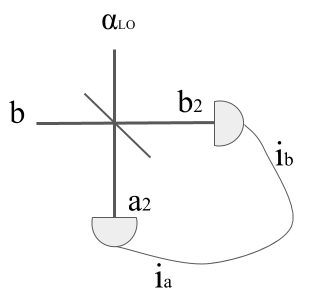
\includegraphics[trim = 0cm 0cm 0cm 0cm, clip, width=0.6\linewidth]{homodyne.png}
\caption{\label{fig:homodyne} Schematic for balanced homodyne detection.}
\end{figure}
In order to detect a quadrature of the mode $ b$, it must be combined with a strong local oscillator at a $50:50$ beam splitter. The local oscillator is a coherent state $\ket{\alpha_{LO}}$, and can be described by a complex classical amplitude. The input and output modes are described by the relations
\begin{eqnarray}
\hat b_2^\dagger = 1/\sqrt{2}(\hat b^\dagger + \alpha_{LO}^*)\\
\hat a_2^\dagger = 1/\sqrt{2}(\hat b^\dagger - \alpha_{LO}^*)\\
\hat b_2 = 1/\sqrt{2}(\hat b + \alpha_{LO})\\
\hat a_2 = 1/\sqrt{2}(\hat b - \alpha_{LO})
\end{eqnarray}
If we measure the difference in photocurrent (or photon number)
\begin{eqnarray}
i_b - i_a &\propto& b_2^\dagger b_2 - a_2^\dagger a_2 \\
		&=& b^\dagger \alpha_{LO} + b \alpha_{LO}^*.
\label{eq:homodyne}
\end{eqnarray}

\noindent By introducing the phase $\phi$ of the local oscillator, \mbox{$\alpha_{LO} = |\alpha|e^{i\theta}$}, 
the expression in Eq.~\eqref{eq:homodyne} simplifies to 
\begin{eqnarray}
 |\alpha|(b^\dagger e^{i\theta}+ b e^{-i\theta}).
\end{eqnarray}

\noindent We identify that this is the quadrature observable $\hat x^{\theta}$.
% 

With all the tools in hand, we are now ready to look at quantum communication protocols in CV. \cite{bib:PhysRevLett.88.057902}

\section{QKD in CV}
A seminar result in CV is the discovery that coherent states are sufficient to perform quantum key distribution. It relies on the fact that coherent states are nonorthogonal.
Let us now explicitly describe 
the coherent beam protocols of this family: 
\begin{enumerate}
\item Alice
draws two random numbers $x_A$ and $p_A$, with zero mean.
\item  She sends to Bob
the coherent state $\ket{x_A + i p_A }$
\item  Bob randomly chooses
to measure either $X$ or $P$ using homodyne detection. 
\item Using a classical public channel, he informs
Alice about the observable that he measured.  Analogous to the BB84 protocol, half of the key generated by Alice is discarded.
\item Alie keeps the bit string value $x_A$ or $p_A$ which matched Bob's quadratures.
\item
Alice and Bob now share two correlated Gaussian
variables. Then they may use classical protocols, e.g. the “sliced reconciliation”
protocol to transform it into a key bit strings.
\item They use privacy
amplification to distill the private key.
\end{enumerate}


% \section{Dense coding}



\section{Teleportation}
Fig.~\ref{fig:tele}
\begin{widetext}
\begin{figure}[h!]
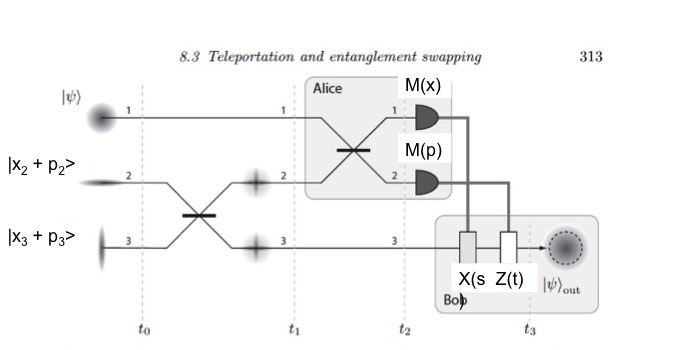
\includegraphics[trim = 0cm 0cm 0cm 0cm, clip, width=1.6\linewidth]{teleport.jpg}
\caption{\label{fig:tele}}
\end{figure} 


\end{widetext}


Protocol extended to CV by \cite{bib:PhysRevA.49.1473, bib:PhysRevLett.80.869}

\cite{bib:kok2010introduction}
\begin{align}
\ket{p} = \int dx e^{i/\hbar p x} \ket{x}, \qquad 
\ket{x} = \int dx e^{i/\hbar x p} \ket{p}
\end{align}

Displacement operator


\begin{eqnarray}
X(s) &=& e^{-i/\hbar x \hat p}\\
X(s)\ket{x} &=&  \int dp e^{-i/\hbar p x} e^{-i/\hbar x \hat p} \ket{p} \\
   			&=& dp e^{-i/hbar p(x+s)} \ket{p} \\
   			&=&\ket{x+s}
\end{eqnarray}

This is the continuous-variable generalization of the Pauli X operator, in that it displaces the value of the state by amount $s$.


The analogue of the Pauli Z operator adds a state-dependent phase
% 
\begin{eqnarray}
Z(t ) &=& e^{i/\hbar t \hat x} \\
 e^{i/\hbar t \hat x} \ket{x} &=& e^{i/\hbar p x} \ket{x}
\end{eqnarray}

\noindent and acts on the momentum basis state $\ket{p}$ as
\begin{eqnarray}
Z(t)\ket{p}=\ket{p+t}.
\end{eqnarray}




Before the squeezing operator is applied, we set $t=0$.
\begin{enumerate}
\item At $t=t_0$, the vacuum states in mode 2 and 3 are squeezed. The quadrature operators become
\begin{align}
x_2(t_0) \rightarrow x_2(0) e^{r} \qquad p_2 \rightarrow p_2(0) e^{-r} \\
x_3(t_0) \rightarrow x_3(0) e^{r} \qquad p_3 \rightarrow p_3(0) e^{-r}
\end{align}
% 
\item The 50:50 beam splitter in modes 2 and 3 creates the approximate
Bell state necessary for teleportation, and this induces the quadrature
transformations
\begin{align}
x_2 (t_1) = \frac{x_2(t_0) + x_3(t_0)}{\sqrt 2} \qquad x_3 (t_1) = \frac{x_2(t_0) - x_3(t_0)}{\sqrt 2} \nonumber\\
p_2 (t_1) = \frac{p_2(t_0) + p_3(t_0)}{\sqrt 2} \qquad p_3 (t_1) = \frac{p_2(t_0) - p_3(t_0)}{\sqrt 2}
\end{align}
\item The second beam splitter induces the transformation
\begin{align}
x_1 (t_2) &= \frac{x_1(t_1) - x_2(t_1)}{\sqrt 2} \\
		  &= \frac{x_1(t_1)}{\sqrt 2} - \frac{x_2(t_0) + x_3(t_0)}{2} \label{b1}\\
% x_2 (t_2) &= \frac{x_1(t_1) - x_2(t_1)}{\sqrt 2} \nonumber\\
		  % &= \frac{x_1 (t_0)}{\sqrt 2} +  \frac{x_2(t_0) + x_3(t_0)}{ 2} label{b1} \\
% p_1 (t_2) &= \frac{p_1 (t_1) + p_2(t_1)}{\sqrt 2} \nonumber \\
p_2 (t_2) &= \frac{p_1(t_1) + p_2(t_1)}{\sqrt 2} \\
		  &=\frac{p_1 (t_0)}{\sqrt 2} +  \frac{p_2(t_0) + p_3(t_0)}{ 2} 
\end{align}
% 

\noindent Now, if we rearrange Eq.~\eqref{b1} to make $x_2(t_0)$ the subject, and identify that $x_1(t_1) = x_1 (t_0)$
\begin{align}
x_2(t_0) &= -2 x_1(t_2)+ \sqrt 2x_1(t_1) - x_3(t_0) \\
		% &= -2 x_1(t_2)+ \sqrt 2x_1(t_0) - x_3(0) e^{-r} \\
p_2(t_0) &= -  2p_2(t_2)  + \sqrt 2 p_1 (t_0) - p_3 (t_0)
\end{align}

\color{blue}
 Now, for Bob, $x_3(t_2) = x_3 (t_1),p_3(t_2) = p_3 (t_1)$, whose state is now
\begin{align}
 x_3 (t_2) &= \frac{-2 x_1(t_2)+ \sqrt 2x_1(t_1) - x_3(t_0) - x_3(t_0)}{\sqrt 2} \nonumber\\
		   &= -\sqrt 2 x_1(t_2 ) + x_1(t_0) - \sqrt 2 x_3(0)e^{-r} \\
 % \frac{2 x_2(t_2)- \sqrt 2x_1(t_0) - x_3(t_0) - x_3(t_0)}{\sqrt2}\\
p_3 (t_2) &=   \frac{p_2(t_0) - p_3(t_0)}{\sqrt 2} \\
		  &=   \frac{-  2p_2(t_2)  + \sqrt 2 p_1 (t_0) - p_3 (t_0) - p_3(t_0)}{\sqrt 2} \\
		  &=  p_1(t_0)- \sqrt2p_2(t_2) - \sqrt2 p_3 (t_0)
\end{align}

\item Alice measures the position quadrature $x_1(t_2)$ in mode 1, yielding
the outcome $s/\sqrt2$, and she measures the momentum quadrature
$p_2(t_2)$ in mode 2, yielding the outcome $t/\sqrt2$. She sends these measurement outcomes to Bob.
\noindent applies the displacements
\begin{align}
X(u) = \exp(-2 i s \hat p_3) \qquad Z(t) = \exp(2i t \hat x_3)
\end{align}
The output quadratures at Bob's mode become
\begin{align}
x_3 = x_1 -\frac{\sqrt2 x_3}{e^r} \qquad p_3 = p_1 - \frac{\sqrt2 p_3}{e^r}
\end{align}
\end{enumerate}

Here the input quadratures are teleported to the output quadratures up to a factor $\frac{\sqrt2 p_3}{e^r}$. In the limit of infinite squeezing $\rightarrow \infty$, the teleportated state is perfect.



\section{Entanglement swapping}

\section{Entanglement distillation}

Entanglement distribution between distant parties is an essential component to most quantum communication protocols \cite{bib:PhysRevLett.81.5932}. As it has been discussed, entanglement is a resource in a quantum network, and it is of interest for distant parties to share maximally entangled states. 

In practice the transmission channel is never perfect, and noise due to interaction with the environment or imperfect gate operations will reduce the entanglement of a state. If one has several copies of some less than maximally entangled state available, it is possible for two parties to concentrate or distill the entanglement.

In contrast to the qubit version, however, it has been proven that for Gaussian states
it is impossible to distill more entanglement by using Gaussian operations \cite{bib:PhysRevLett.89.137904, bib:PhysRevLett.89.137903, bib:PhysRevA.66.032316}. In order to to distill from Gaussian input states, non-Gaussian operations are necessary.
 
Proposal \cite{bib:eisert2004distillation}, one variant experimentally realized by photon-subtraction \cite{bib:takahashi2010entanglement}.

\section{Quantum computing}



\subsection{Quantum gates}

Gates for the qubit circuit model and the analogous operations for CV are summarised in Table~\ref{tabgates}. \cite{bib:RevModPhys.84.621}
\begin{table}
\begin{tabular}{ |c|c| } 
 \hline
 Circuit model &  CV cluster state \\ 
  \hline\hline
 Pauli $X$ & $X(s) = \exp[-i s \hat p]$  \\ 
 Pauli $Z$ & $Z(t) = \exp[i t \hat q]$  \\ 
 Phase gate & $\hat P (\eta) = \exp[i \eta \hat x^2]$ \\
Hadamard   & $F=\exp[i \frac{\pi}{8}(\hat p^2+\hat q^2)]$ \\
$C_Z$	   & $C_Z= \exp[\frac{i}{2}q_1 \otimes q_2]$ \\
CNOT 	   & $C_X = \exp[-2i\hat x_1 \otimes \hat p_2]$\\
\hline
\end{tabular}
\caption{\label{tabgates}}
\end{table}
%  

The operators $X,Z$ can be interpreted as displacement operators
\begin{align}
D(\alpha) = \exp(\alpha \hat a^\dagger - \alpha^* \hat a)
\end{align}
which correspond to a translation in phase space. $X$ is a translation in position, and Z is a displacement in momentum.

The X and Z operators can be written as 
X = D(s/2), Z = D(it/2)



The Fourier gate F is the Gaussian analogue of the qubit Hadamard gate, which corresponds to a $\pi/2$ rotation in phase space, and transforms the quadrature eigenstates from one to another:

\begin{eqnarray}
F = \exp(i\pi/4)\exp(\frac{i\pi}{4} \hat a^\dagger \hat a) = (\hat p^2+\hat x^2)
\end{eqnarray}

\begin{eqnarray}
F\ket{s}_x = \ket{s}_p
\end{eqnarray}


The controlled-phase gate, $C_Z$ is a two-mode Gaussian gate. It is defined as

\begin{eqnarray}
E_z = \exp\left(\frac{i}{2} \hat x_1 \otimes \hat x_2 \right).
\end{eqnarray}

It transforms on the quadrature eigenstates as
\begin{eqnarray}
C_Z \ket{s}_1 \ket{t}_2 = \exp(i s_1 t_2)/2 \ket{s}_1\ket{t}_2  
\end{eqnarray}


It transforms the momentum quadratures according to

\begin{eqnarray}
\hat p_1 \rightarrow \hat p_1 + \hat x_2, \qquad \hat p_2 \rightarrow \hat p_2 + \hat x_1
\end{eqnarray}

\subsection{Cluster state/ measurement based}



\cite{bib:PhysRevLett.97.110501}
The advantage of this approach is that both the cluster state preparation and commutation can be performed deterministically.

Once the state has been created, a sequence of one-mode (separable) measurement 


The one-qubit teleportation give insight into how the cluster-state evolves in this model


\begin{figure}
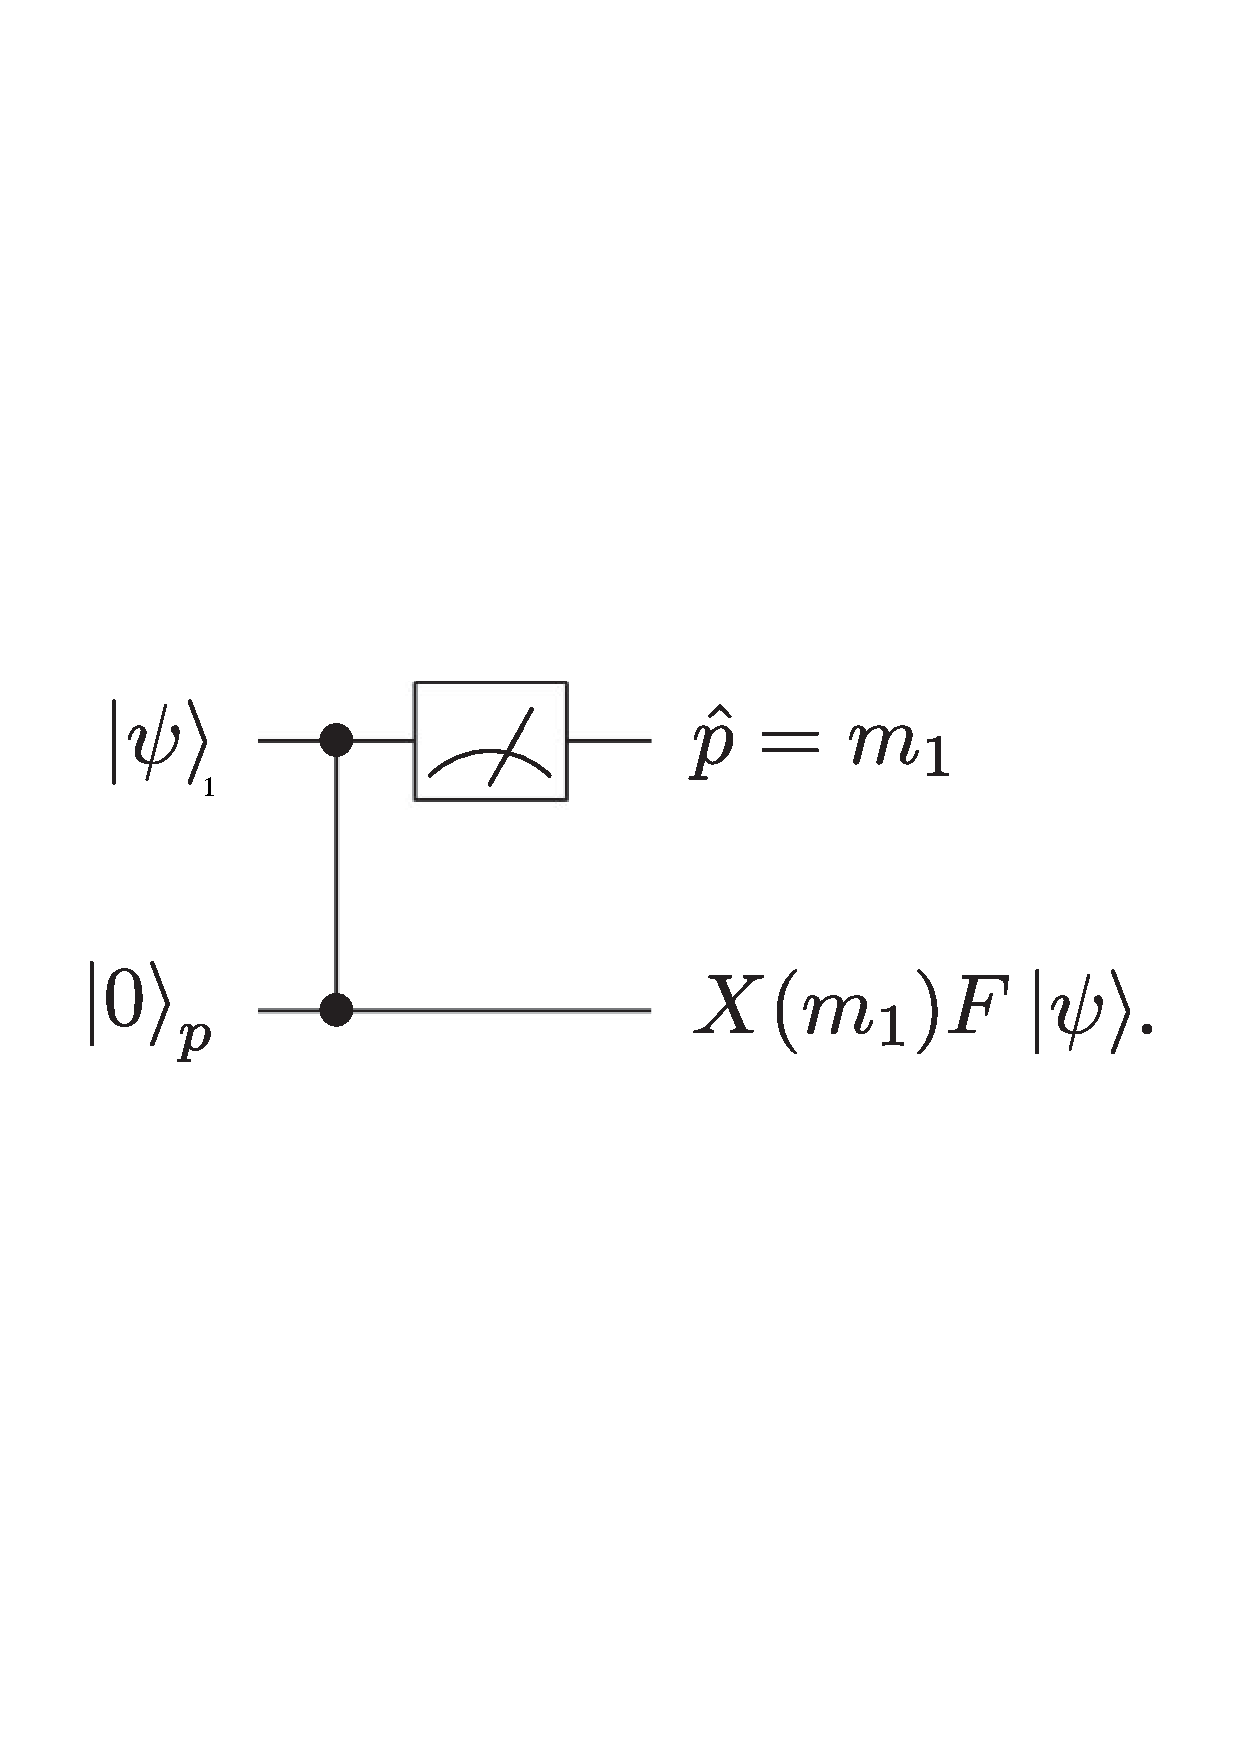
\includegraphics[trim = 0cm 10cm 0cm 10cm, clip, width=0.75\linewidth]{one_qubit_teleport.pdf}
\caption{\label{fig:cluster_Teleport}}
\end{figure}

 Consider perfect squeezing, where the second mode is a momentum eigenstate $\ket{0}_p$. Initially, the state is 


\begin{eqnarray}
\ket{\psi}\ket{0}_p = \frac{1}{\sqrt {2\pi}} \int dx_1 dx_2 \psi(x_1)\ket{x_1}\ket{x_2}
\end{eqnarray} 

Applying the $C_Z$ gate results in


\begin{eqnarray}
\frac{1}{2\pi} \int dx_1 dx_2 \psi(x_1) \exp(i x_1 x_2/2)\ket{x_1}\ket{x_2}
\end{eqnarray}

After measuring $\hat p_1$, the state is projected onto $\ket{m_1}\bra{m_1}$, we have

$\braket{m_1|q_1}= 1/2\pi \exp(-iq_1 m_1/2)$


\begin{eqnarray}
\frac{1}{4\pi}\int d x_1 d x_2 \psi(x_1) \exp(i x_1 (q_2 - m_1)) q_2
 \end{eqnarray}
 
Applying the correction $X(m_1)$ gives back the initial state $\ket{\psi}$

% \begin{enumerate}
% 	\item
% 	\item mode 1 and 2 are entangled using a $C_Z$  gate
% 	\item Measurement in $\hat p$ is performed on mode 1, resulting in outcome $m_1$
% \end{enumerate}

We can now consider the teleportation of a quantum gate, which is the key of the measurement-based quantum computing.
Consider a variation of the above circuit, where the only difference is the addition of a unitary that is diagonal 
in the computational basis, and therefore commutes with the CPHASE gate, for example $U=\exp(i f(\hat x))$. 


\begin{figure}[thb]
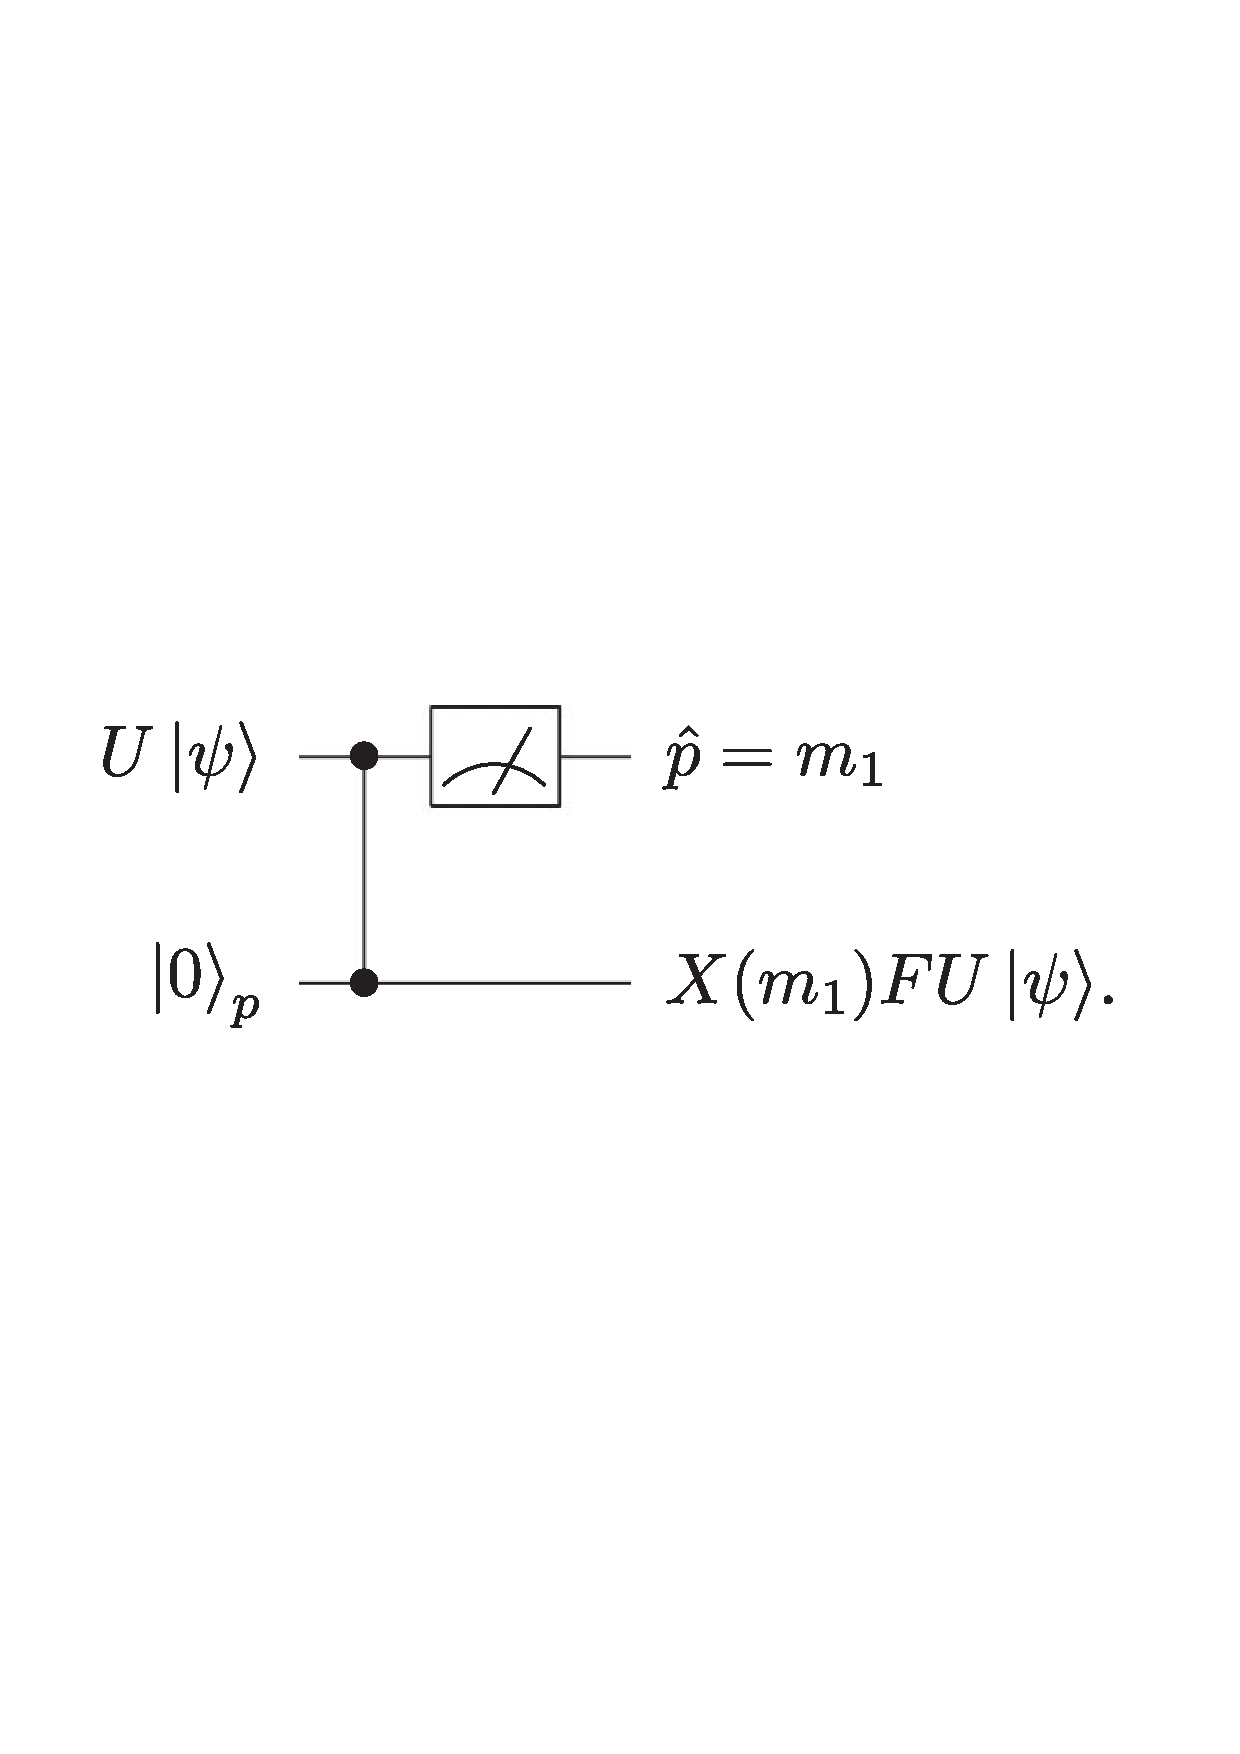
\includegraphics[trim = 0cm 10cm 0cm 10cm, clip, width=0.8\linewidth]{teleport_circ2.pdf}
\\
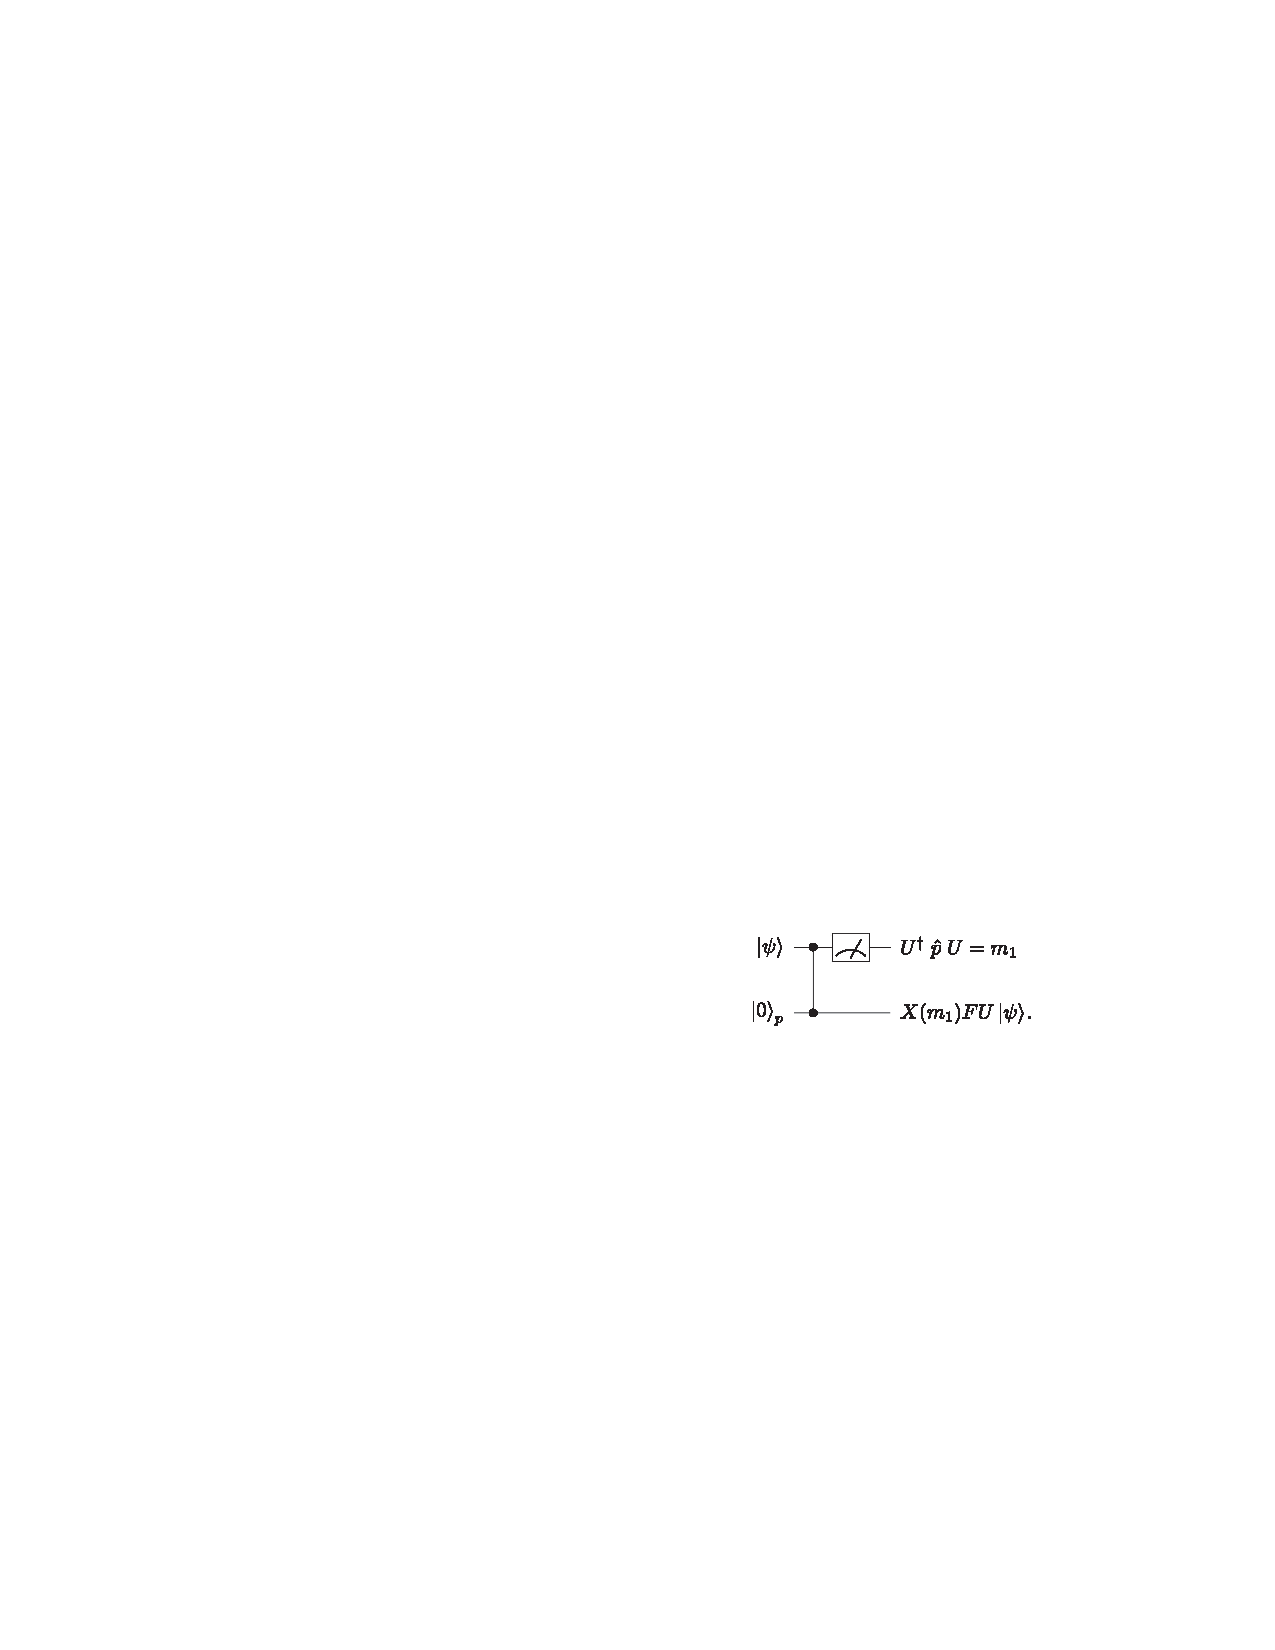
\includegraphics[trim = 0cm 0cm 0cm 0cm, clip, width=0.8\linewidth]{teleport_circ3.pdf}
\caption{\label{fig:cluster_Teleport23}}
\end{figure}




We have just shown that 
by performing a measurement in the basis $U\hat x U^\dagger$, we can absorb the gate into the measurement. 

% \section{}
\begin{itemize}
	\item addition of any non-gaussian projective measurement allows universal QC using CV cluster states
	\item multimode Gaussian operations can be made in any order
\end{itemize}

\bibliography{reference}

\end{document}